\chapter{Unsafe Rust and FFI}

\section{Breaking the Rules (Carefully): The Need for Unsafe Rust}

Throughout this book, you have seen how Rust's borrow checker and strict ownership rules prevent a myriad of memory safety issues at compile time. Safe Rust is designed to systematically eliminate \textbf{undefined behaviors (UBs)}. This does not merely refer to memory mismanagement (such as dereferencing a pointer that has already been freed), but also extends to concurrency issues, like preventing two threads from incrementing the same shared variable without synchronization (data races).

By default, the compiler is incredibly conservative: if it cannot guarantee with absolute certainty that a piece of code is safe, it will reject it. While this conservatism is the cornerstone of Rust's reliability, it occasionally poses a problem. Sometimes, you know a specific memory manipulation is valid, but you cannot express those invariants in a way the compiler understands. 

Furthermore, systems programming does not happen in a vacuum. Operating systems are often written in C, and you will frequently need to interact with hardware directly or call existing C libraries. Hardware and C compilers do not understand Rust's borrowing rules. 

To solve these problems, Rust provides an escape hatch: \textbf{Unsafe Rust}. By using the \texttt{unsafe} keyword, you temporarily take over the responsibility of ensuring memory safety from the compiler. You are telling the compiler, "Trust me, I know what I am doing." 

\begin{examprioritybox}
As the professor often highlights, the language intentionally forces you to be verbose when bypassing its protections. When you need to deliberately bypass the borrow checker (for example, to demonstrate a data race manually), you find yourself having to write \texttt{unsafe} multiple times, wrapping structures like \texttt{UnsafeCell} in \texttt{unsafe} blocks. This verbosity is by design: it serves as a repeated, explicit acknowledgment where you declare, ``Yes, I am violating the rules; yes, I know I am overriding the safeguards built to prevent undefined behaviors; I take full responsibility.''

\textbf{Common Pitfall:} Thinking that a single \texttt{unsafe} block turns off the borrow checker globally. It does not; it only allows specific unsafe operations, and you still have to manually prove to yourself that you aren't causing undefined behaviors like data races.

\textbf{Expected Mastery Level:} High. You must understand exactly why the language forces this verbosity and what responsibilities you take on when using \texttt{unsafe}, especially when manipulating shared state.
\end{examprioritybox}

\begin{insightbox}
\textbf{What Unsafe Rust Does NOT Do}\\
A common misconception is that \texttt{unsafe} turns off the borrow checker entirely. This is false. Inside an \texttt{unsafe} block, references are still checked, and ownership rules still apply. The \texttt{unsafe} keyword simply unlocks five specific "superpowers":
\begin{itemize}
    \item Dereference a raw pointer.
    \item Call an unsafe function or method.
    \item Access or modify a mutable static variable.
    \item Implement an unsafe trait.
    \item Access fields of \texttt{union}s.
\end{itemize}
Everything else remains strictly checked.
\end{insightbox}

\section{Raw Pointers: Bypassing the Borrow Checker}

The most common reason to use Unsafe Rust is to manipulate \textbf{raw pointers}. While Rust's standard references (\texttt{\&T} and \texttt{\&mut T}) are guaranteed to be valid and non-aliasing, raw pointers (\texttt{*const T} for immutable and \texttt{*mut T} for mutable) are much more akin to C pointers. 

Raw pointers have very different rules compared to standard references:
\begin{itemize}
    \item They are allowed to ignore borrowing rules by having both mutable and immutable pointers to the same memory location, or multiple mutable pointers.
    \item They aren't guaranteed to point to valid memory (they can be null or dangling).
    \item They don't implement automatic cleanup (no \texttt{Drop}).
\end{itemize}

\subsection{Creating and Dereferencing Raw Pointers}

You can \textit{create} raw pointers in safe code. The compiler does not mind if you simply hold a raw pointer; the danger only arises when you try to read from or write to the memory it points to. Therefore, \textit{dereferencing} a raw pointer requires an \texttt{unsafe} block.

Let's look at a concrete example of creating raw pointers from standard references:

\begin{lstlisting}[language=Rust]
fn main() {
    let mut num = 5;

    // Creating raw pointers is SAFE
    let r1 = &num as *const i32;
    let r2 = &mut num as *mut i32;

    // Dereferencing raw pointers is UNSAFE
    unsafe {
        println!("r1 is: {}", *r1);
        *r2 = 10;
        println!("r2 modified num to: {}", *r2);
    }
}
\end{lstlisting}

\textbf{When and Why to Use It:} Use raw pointers when you are interfacing with C code that expects pointers, or when you are building foundational data structures (like a doubly-linked list or a custom \texttt{Vec}) where you must bypass the strict aliasing rules of safe Rust.

\textbf{Deep Memory Model Analysis:}
In the snippet above, \texttt{num} is a local variable allocated on the stack. Because it is an \texttt{i32}, it occupies 4 bytes of stack space. When we create \texttt{r1} and \texttt{r2}, no new heap allocations occur, and no ownership is transferred; we are merely creating stack-allocated raw pointers (memory addresses) that point back to the stack location of \texttt{num}. Safe Rust borrowing rules usually prevent the existence of simultaneous mutable and immutable references. However, by casting to raw pointers (\texttt{*const i32} and \texttt{*mut i32}), we circumvent the borrow checker's aliasing guarantees. The lifetimes of raw pointers are not tracked by the compiler, meaning they could outlive \texttt{num} and become dangling. Here, it is safe because the operations occur within \texttt{main} where \texttt{num} is guaranteed to be valid, but the \texttt{unsafe} block is necessary for the compiler to allow dereferencing.

In this code, we cast a valid reference to a raw pointer. Because we know \texttt{num} lives for the entire duration of \texttt{main}, we can safely assure ourselves that dereferencing \texttt{r1} and \texttt{r2} will not result in a segmentation fault. However, the compiler cannot prove this via the raw pointers, so it requires the \texttt{unsafe} block.

\begin{notebox}
\textbf{Visualizing Memory Layout}\\
To better conceptualize how unsafe code maps to system memory, it is helpful to look at how raw pointers operate under the hood. Refer to \textbf{Figure~\ref{fig:unsafe_rust}} (\texttt{images/unsafe\_rust.png}), which illustrates how raw pointers can bypass the typical stack guarantees and point directly to arbitrary heap segments or memory-mapped I/O registers.
\end{notebox}

\begin{figure}[ht]
    \centering
    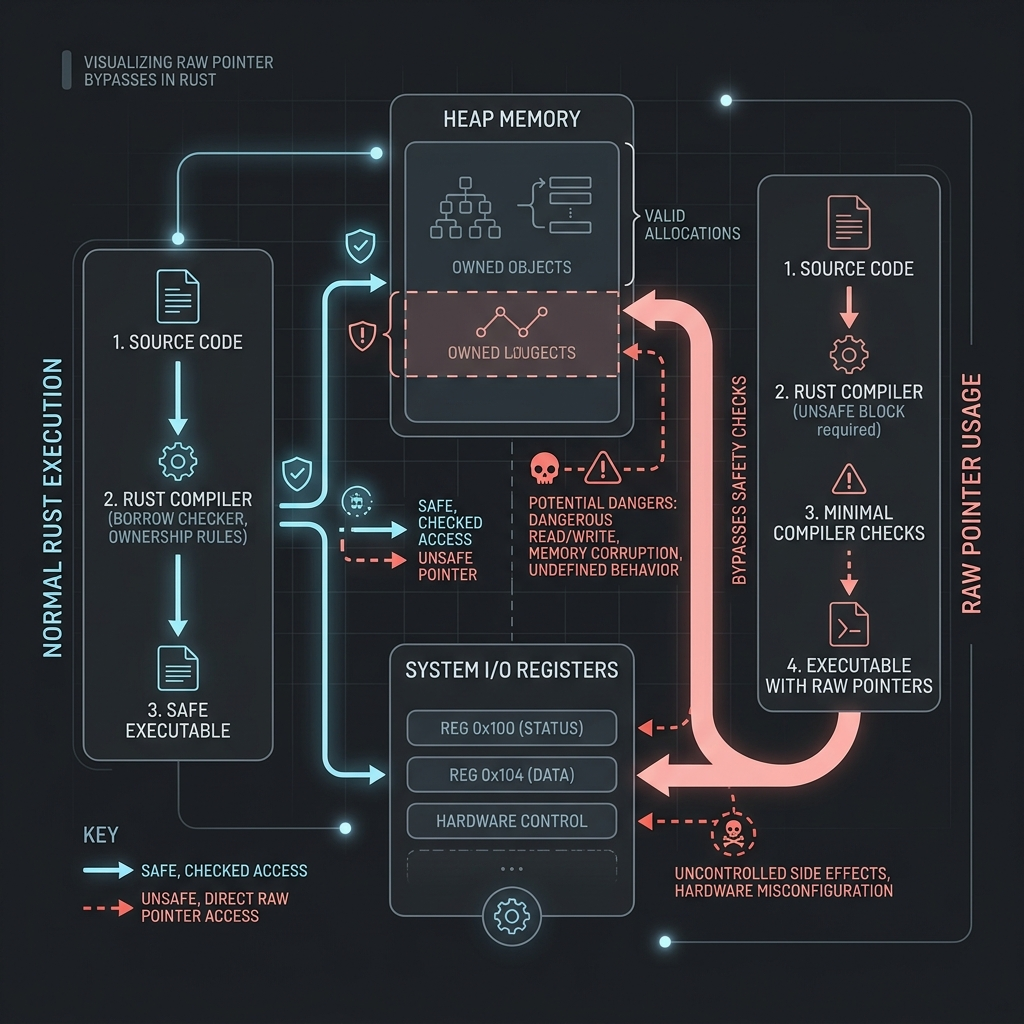
\includegraphics[width=0.8\textwidth]{images/unsafe_rust.png}
    \caption{Visualizing raw pointer bypasses in Rust}
    \label{fig:unsafe_rust}
\end{figure}

\section{Unsafe Functions and Safe Abstractions}

You can declare an entire function as unsafe by prefixing it with the \texttt{unsafe} keyword. This means the function has internal requirements that the compiler cannot verify, and the caller must ensure these conditions are met before calling it. Calling an \texttt{unsafe fn} must always be done inside an \texttt{unsafe} block.

\begin{lstlisting}[language=Rust]
unsafe fn dangerous_operation() {
    // This function performs unchecked memory operations
}

fn main() {
    unsafe {
        dangerous_operation();
    }
}
\end{lstlisting}

\subsection{The Philosophy of Safe Abstractions}

One of the most important architectural patterns in Rust systems programming is building \textbf{safe abstractions over unsafe code}. Just because your library uses \texttt{unsafe} internally doesn't mean your users should have to write \texttt{unsafe} blocks. If you can wrap the unsafe operations in a safe function API that meticulously enforces the necessary invariants, you can expose a completely safe interface.

A classic example is the standard library's \texttt{split\_at\_mut} method for slices. It takes a mutable slice and splits it into two non-overlapping mutable slices. The compiler's borrow checker isn't smart enough to know that the two resulting slices don't overlap, so the implementation uses \texttt{unsafe} pointer math. However, the method signature itself is completely safe, meaning users can call it without \texttt{unsafe} blocks.

Another crucial example of this philosophy is \textbf{interior mutability}. Types like \texttt{Cell}, \texttt{RefCell}, and \texttt{Mutex} provide a safe API to mutate data through a shared reference. Under the hood, however, they all rely on \texttt{std::cell::UnsafeCell}, the core primitive in Rust that legally bypasses the borrow checker to allow mutating data across an immutable reference. By wrapping \texttt{UnsafeCell} and enforcing runtime checks or thread synchronization, these types expose a safe interface over an inherently unsafe operation.

\textbf{When and Why to Use It:} Create safe abstractions over unsafe code when you are writing a library or a core component that needs maximum performance or hardware access, but you want to expose a foolproof, safe API to the rest of the application.

\subsection{Unsafe Traits: Send and Sync}

One of the five "superpowers" of Unsafe Rust is the ability to implement an \texttt{unsafe trait}. The most prominent examples of unsafe traits in Rust are the concurrency marker traits: \textbf{\texttt{Send}} and \textbf{\texttt{Sync}}.

\begin{itemize}
    \item \textbf{\texttt{Send}} indicates that ownership of a value of this type can be safely transferred to another thread.
    \item \textbf{\texttt{Sync}} indicates that it is safe for multiple threads to hold immutable references (\texttt{\&T}) to a value of this type simultaneously. A type \texttt{T} is \texttt{Sync} if and only if \texttt{\&T} is \texttt{Send}.
\end{itemize}

These are \textbf{marker traits}, meaning they have no methods. The Rust compiler automatically implements them for most types if all their constituent parts are also \texttt{Send} and \texttt{Sync}. However, if you are building a custom concurrency primitive (or intentionally bypassing safety), you might need to implement them manually. Because the compiler cannot verify thread-safety guarantees on its own when raw pointers or interior mutability are involved, \texttt{Send} and \texttt{Sync} are marked as \texttt{unsafe trait}s. Implementing them requires an \texttt{unsafe impl} block, whereby you, the programmer, take full responsibility for ensuring the absence of data races.

\subsection{Demonstrating Undefined Behavior: Forcing a Data Race}

To truly appreciate the protections Safe Rust offers, we can look at what it takes to deliberately create a data race. As the professor detailed in the lecture, if you want to demonstrate a classic read-modify-write data race (e.g., two threads incrementing the same variable), you have to fight the compiler every step of the way. 

You must manually bypass the protections by creating a custom structure, wrapping the data in an \texttt{UnsafeCell}, and explicitly forcing the \texttt{Sync} trait implementation.

\begin{lstlisting}[language=Rust]
use std::cell::UnsafeCell;
use std::thread;

// 1. Create a custom structure wrapping UnsafeCell
struct MyUnsafeCounter {
    value: UnsafeCell<i32>,
}

// 2. Implement an unsafe trait. We force the compiler to trust us!
// Without this, we cannot share MyUnsafeCounter across threads.
unsafe impl Sync for MyUnsafeCounter {}

impl MyUnsafeCounter {
    fn process(&self) {
        // 3. Unsafe block required to dereference the raw pointer from UnsafeCell
        unsafe {
            let before = *self.value.get();
            *self.value.get() = before + 1;
            let after = *self.value.get();
            
            let delta = after - before;
            if delta != 1 {
                // This will print due to the data race!
                println!("Delta is negative or strange: {}", delta); 
            }
        }
    }
}

fn main() {
    // Variable instantiated in main, shared by reference
    let counter = MyUnsafeCounter { value: UnsafeCell::new(0) };

    thread::scope(|s| {
        // Spawn two threads, each doing 10 million iterations
        s.spawn(|| {
            for _ in 0..10_000_000 { counter.process(); }
        });
        s.spawn(|| {
            for _ in 0..10_000_000 { counter.process(); }
        });
    });
}
\end{lstlisting}

\textbf{Step-by-step Walkthrough:}
\begin{enumerate}
    \item \textbf{Custom Structure and \texttt{UnsafeCell}:} The compiler normally prevents mutating shared data. By using \texttt{UnsafeCell}, we get a raw pointer to the inner data, enabling interior mutability.
    \item \textbf{\texttt{unsafe impl Sync}:} Because \texttt{UnsafeCell} is expressly \textit{not} thread-safe, it does not implement \texttt{Sync}. To pass our \texttt{MyUnsafeCounter} across threads, we must implement \texttt{Sync} manually. We use \texttt{unsafe impl}, effectively telling the compiler: "I take full responsibility for thread safety."
    \item \textbf{The \texttt{unsafe} Block:} Inside the \texttt{process} method, calling \texttt{self.value.get()} returns a raw pointer (\texttt{*mut i32}). Dereferencing this raw pointer to read \texttt{before}, increment, and read \texttt{after} requires an \texttt{unsafe} block.
\end{enumerate}

\begin{insightbox}
\textbf{The Professor's Analogy: "I violate all the rules"}\\
When demonstrating this data race, the professor highlights how much effort it takes to create undefined behavior in Rust: \textit{``You see how many times it has to say: 'I violate all the rules.' Because it's built to prevent us from doing it. So I had to say it a million times: 'Yes, Unsafe, Unsafe, I know, Unsafe is wrong. Yes, I know, I know, I know.' Patience, right?''}

The verbosity of Unsafe Rust is a feature, not a bug. It ensures that undefined behaviors, such as read-modify-write data races that lead to lost updates or bizarre negative deltas, are never introduced accidentally.
\end{insightbox}

\begin{warningbox}
\textbf{Undefined Behaviors and Concurrency}\\
Undefined behaviors (UBs) do not just mean dereferencing a freed pointer (use-after-free). As the professor stressed, \textbf{two threads incrementing the same shared variable} is an intrinsic concurrency problem that triggers UB. In a data race, a thread might be suspended mid-operation (e.g., after reading 5 but before writing 6). When it wakes up, it overwrites the progress made by other threads, resulting in lost increments and a final counter well below the expected 20 million.
\end{warningbox}

\begin{insightbox}
\textbf{The Professor's Analogy: The Fridge and TOCTOU}\\
The core issue behind data races is \textbf{TOCTOU} (Time Of Check to Time Of Use). The professor uses a vivid analogy: \textit{``Before, in the fridge, there was my lunch. When I needed it, there was no more.''} 

You cannot assume that shared things remain exactly as they were when you last checked them. If you read a value (Time of Check) and then are suspended by the scheduler, by the time you wake up and write the modified value (Time of Use), another thread may have already altered the state, making your original read obsolete.
\end{insightbox}

\section{Foreign Function Interface (FFI)}

A primary motivation for Unsafe Rust is interacting with other languages, particularly C. This is known as a Foreign Function Interface (FFI). Because C does not respect Rust's borrow checker or memory models, crossing the boundary between Rust and C is inherently unsafe.

\subsection{Calling C from Rust}

Suppose you are building an application and need to rely on a heavily optimized, pre-existing C library. Rewriting it in Rust would be too costly and error-prone. Instead, you can define the C functions in Rust using an \texttt{extern} block and call them directly.

\begin{lstlisting}[language=Rust]
// We define the signature of the C standard library's 'abs' function
extern "C" {
    fn abs(input: i32) -> i32;
}

fn main() {
    let x = -3;
    // Calling an external function is inherently unsafe
    unsafe {
        println!("Absolute value of {} according to C is: {}", x, abs(x));
    }
}
\end{lstlisting}

\textbf{When and Why to Use It:} Use FFI when you need to leverage existing C/C++ libraries (e.g., standard libraries, system calls, optimized math routines) without rewriting them in Rust.

\textbf{Deep Memory Model Analysis:}
When calling \texttt{abs(x)}, the Rust compiler places \texttt{x} (an \texttt{i32}) in a CPU register or on the stack according to the C Application Binary Interface (ABI) conventions for the target platform. Ownership is implicitly handled by copying, since \texttt{i32} implements \texttt{Copy}. The C function executes entirely outside of Rust's memory model; it manages its own stack frame. Once the C function returns, the integer result is placed back into the expected return register (like \texttt{rax} or \texttt{eax} on x86) and read by the Rust runtime. Because the Rust compiler cannot track what the C function does with memory, the call is intrinsically \texttt{unsafe}.

The \texttt{"C"} specifies the \textbf{Application Binary Interface (ABI)}. The ABI defines how the function is invoked at the assembly level (how arguments are passed, how the stack is managed). The C ABI is the \textit{lingua franca} of systems programming.

\begin{warningbox}
\textbf{The Danger of FFI}\\
When calling C code, the Rust compiler completely trusts the signature you provide in the \texttt{extern} block. If you incorrectly define a C function as taking an \texttt{i32} when it actually takes an \texttt{i64}, or if the C function corrupts the stack, the Rust compiler cannot save you. Your program will crash or exhibit undefined behavior.
\end{warningbox}

\subsection{Calling Rust from C}

The relationship goes both ways. You can expose Rust functions so they can be compiled into a shared library and called by C, Python, Node.js, or any language that supports the C ABI.

To do this, you must instruct the Rust compiler not to "mangle" the function name. Name mangling is a technique compilers use to add extra information to function names to support features like namespaces and generics. Since C does not support mangling, we disable it using the \texttt{\#[no\_mangle]} attribute.

\begin{lstlisting}[language=Rust]
#[no_mangle]
pub extern "C" fn call_from_c() {
    println!("Just called a Rust function from C!");
}
\end{lstlisting}

\textbf{Deep Memory Model Analysis:}
By marking the function with \texttt{\#[no\_mangle]} and \texttt{extern "C"}, we instruct the Rust compiler to export the symbol exactly as \texttt{call\_from\_c} and to expect arguments and return values using the C stack/register conventions. When a C program calls this function, the transition crosses the ABI boundary: the C stack frame is prepared, and execution jumps into the Rust compiled code. Inside the function, standard Rust stack allocation and ownership rules resume. The \texttt{println!} macro allocates temporary structures on the stack and safely borrows the string slice. 

This function can now be exported as a standard C symbol. Notice that \texttt{unsafe} is not required on the Rust side here, as the Rust code itself obeys all safe rules. The unsafety is offloaded to the C code that calls it.

\begin{exambox}
\textbf{Exam Tip}\\
Be prepared to explain \textit{why} FFI operations require the \texttt{unsafe} keyword, and how the \texttt{extern "C"} block dictates the ABI. Also, be sure to understand the purpose of \texttt{\#[no\_mangle]} when exposing Rust code to other languages.
\end{exambox}

\section{Trade-offs: Performance vs. Correctness}

Using Unsafe Rust is always a trade-off. By manually managing pointers or hooking into FFI, you gain performance, extreme flexibility, and interoperability. However, you completely forfeit the compiler's safety net for those specific operations. A single mistake in an \texttt{unsafe} block can introduce use-after-free vulnerabilities, buffer overflows, or data races---the exact bugs Rust was designed to eliminate.

Therefore, the golden rule of System Programming in Rust is: \textbf{Keep unsafe blocks as small as possible}. Encapsulate them behind safe, thoroughly-tested abstractions so that the rest of your codebase can remain entirely safe.

\subsection*{Exam Relevance and Recurrence}
\textbf{Score: High}

\textbf{Notes:} FFI and Unsafe Rust are frequent exam topics, particularly the justification for \textit{why} an \texttt{unsafe} block is needed and what it enables. You will likely be asked to explain the relationship between Safe Rust abstractions (like \texttt{UnsafeCell} and \texttt{Mutex}) and Unsafe Rust, and how FFI violates the borrow checker's assumptions. The verbosity of Unsafe Rust in demonstrating race conditions is a recurring conceptual question.

\section{Domande ed Esercizi da Esami Passati}

\textit{Nessuna domanda d'esame specifica presente per questo capitolo.}
